\documentclass{article}

\usepackage[utf8]{inputenc}
\usepackage[icelandic,english]{babel}
\usepackage[T1]{fontenc}
\usepackage{graphicx}
\usepackage{wrapfig}
\usepackage{parskip}
\usepackage{url}
\usepackage{pdfpages}

\graphicspath{{./images/}}

\begin{document}	
	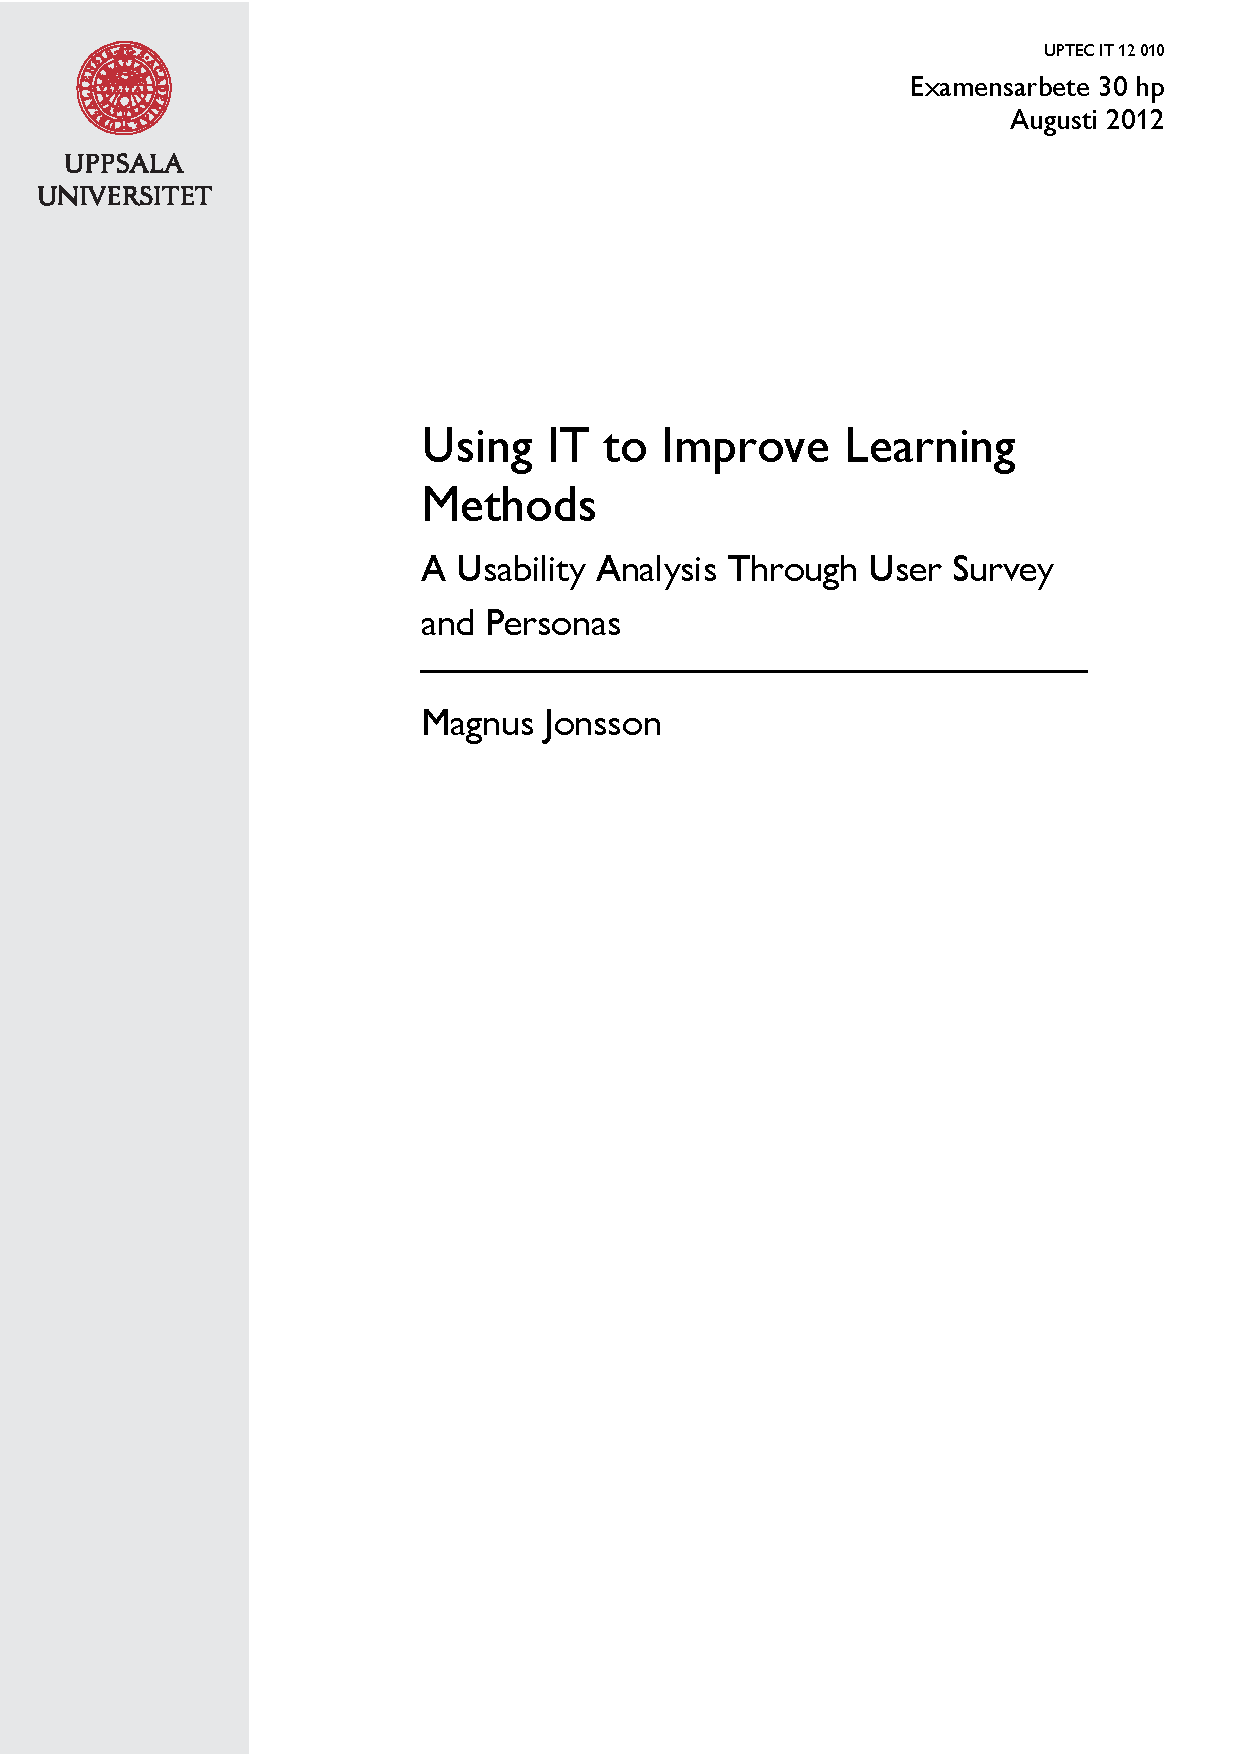
\includepdf[pages={1}]{frontpage.pdf}
	\newpage
	\thispagestyle{empty}
	\mbox{}
  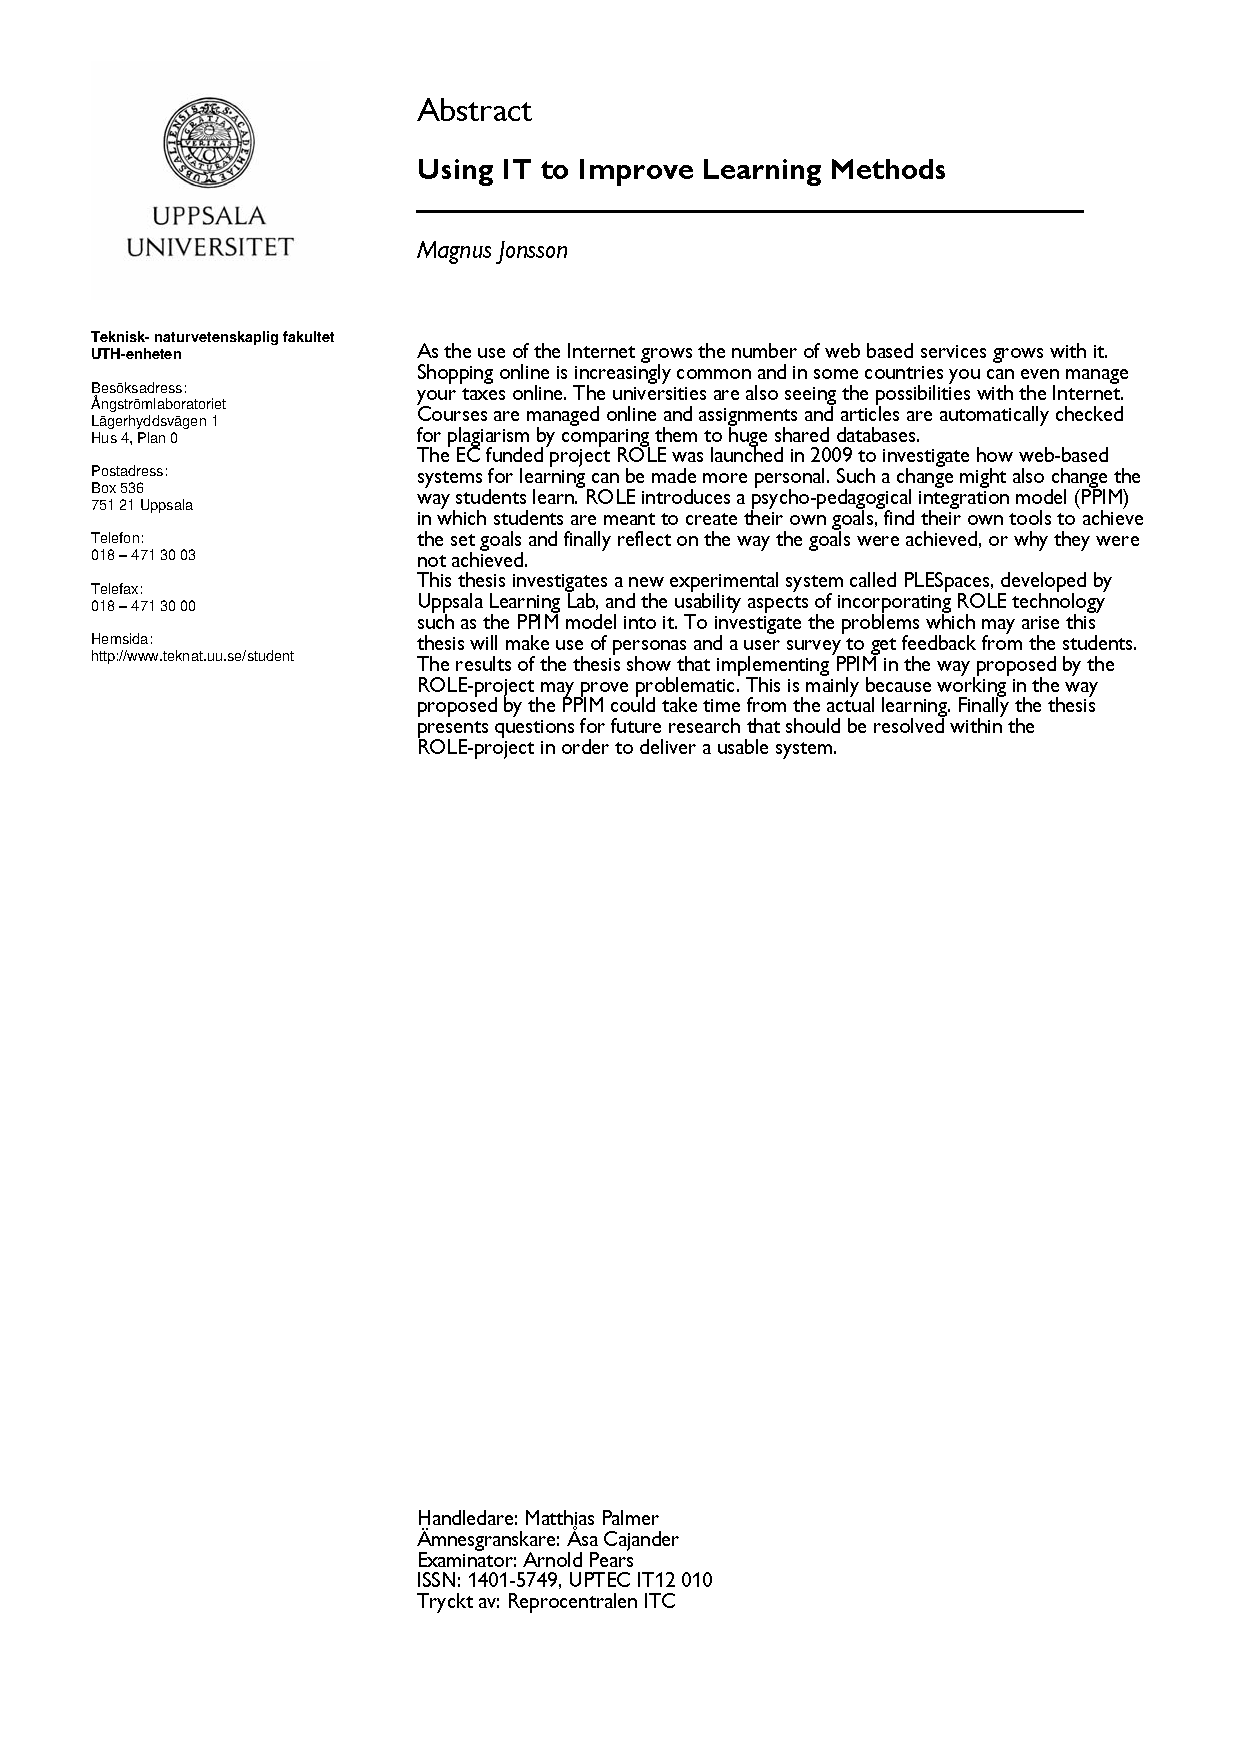
\includepdf[pages={1}]{abstract.pdf}
  \newpage
  \thispagestyle{empty}
	\mbox{}
  \newpage
  \thispagestyle{empty}
	\mbox{}
	\section*{Acknowledgements}
		I would like to thank the following people:
		\begin {itemize}
			\item Mattias Palmer, ULL, My  supervisor at Uppsala Learning Lab - For providing me with everything I needed to complete this thesis.
			\item Erik Isaksson, ULL - For providing me with insights into research done within the ROLE project.
			\item Uppsala Learning Lab - For giving me free roam around your awesome facilities and giving me my own office wh‌en writing this thesis.
			\item Effie Law, ETH Zürich - For providing me with results and insights from previous surveys done within the ROLE project.
			\item Åsa Cajander, Uppsala University, My instructor at Uppsala University - For taking all the time reading this thesis over and over; making sure it is up to academic standards.
		\end {itemize}
	\newpage
	\section*{Reading Instructions}
		This thesis is structured in the following way: First you will be introduced to the problem and also an explaination as to why it is a problem. Later this thesis will explain how the problem was attacked. The next section will feature research related to this problem ans also deeper examination of the methods used in this thesis, followed by the requirements set by different parties. Two sections will follow explaining the actual methods and the results. Finally the results will be analyzed and discussed.
		
		To make this thesis easier to read I have included a guide for those who do not wish to read it from cover to cover:
		If you are interested in the part of the thesis that reflects on the ROLE project you should read the following sections: 1.1 - Background, 2.1-2.3 - Previous Work. 4 - Interaction design. 5.1.2 and 5.2.1 - Usability Recommendations. 6-8: Analysis, Discussion and Future Work.
		If you are a usability expert and wants to know how this method was useful or not I would recommend the following sections: 1 - Introduction. 2.4-2.5 - Personas and Interaction Design. 4-5 - Results from Interaction Design and Usability investigation. 7 - Discussion.
	\newpage
	\tableofcontents
	
	\chapter{Introduction}

\setcounter{section}{2}
\setcounter{subsection}{0}



\subsection{Reading Instructions}

\subsection{Background}

\subsection{Problem}

\subsection{Purpose and Goal}

\subsection{Restrictions}

\subsection{Method}

	\section {Previous Work}
As sir Isaac Newton once said: "If I have seen further it is only by standing on the shoulders of giants." No academic research can be done single handedly. The first part of this section will give a short summary of what has been researched earlier within, or related to, the ROLE-project. These topics include the personal learning environments, widgets and the psycho-pedagogical integration model. The second part will give an introduction to the methods and tools used in this thesis. These topics include interaction design and the use of personas.

\subsection { Personal Learning Environments }
A personal learning environment (PLE) is not an application. A PLE consists of different tools and services used in everyday learning \cite{attwell}. A PLE is as the name suggests personal. In a class of 30 students it is likely to find 30 different learning environments. A common set up is a word processor, a web browser, a mail client and a communication tool. The web browser probably displays multiple web sites including searches for academic research, tools for quickly checking facts and a translating service. All of these programs and websites take a lot of place on the screen, it also takes time to set up. There is also no guarantee that these programs work well together.  It might be preferable if all these tools could be incorporated into one larger system with set standards for synchronizing tools with each other.

Looking at the requirements from the ROLE-project (The full list can be found in the requirements section, section 3.1) we find the following requirements: “ROLE should provide users with the ability to construct and maintain a Personal Learning Environment. (PLE)” and “Inter-tool communication in the PLE” \cite{chatterjee}. This means that the experimental platform PLESpaces should allow students to create a personal learning environment where the tools added should be able to communicate with each other. Within the ROLE-project it has been decided to build systems, like PLESpaces, as a widget space where individual widgets, with widget-communication capabilities, can be added.

A special feature called recommendation service should also be included. This service should analyse the user's behaviour, such as current goals and previous knowledge, and deliver recommendations. These recommendations include tools, complete widget spaces and fellow students for collaboration.

\subsection {Widgets}
Widget is an ambiguous term. The definition according to Cambridge Advanced Learner's Dictionary is  "any small device whose name you have forgotten or do not know" or "an imagined small product made by a company".
In today's world of IT widgets often refer to a small single purpose application that can be attached to a widget area. Widgets are used in systems like Apple's Macintosh Dashboard, Gadgets in Microsoft's Windows Vista and Windows 7 and mobile platforms such as Google's Android. In the ROLE-project and this thesis widgets refers to "small portable Web-enabled applications" that can be run in a web environment. \cite{kiefel}

\subsubsection {OpenApp}
Widgets are allowed to communicate with each other. If an action occurs in one widget (e.g the user makes a selection) another widget could activate and react accordingly (e.g. save information as a bookmark). Within the ROLE-project a framework called OpenApps has been developed \cite{isaksson}. This framework defines how widgets send and receive messages to and from other widgets.

\subsubsection {Widget Space}
Inspired by Google's system iGoogle the ROLE-project has developed the idea that widgets should be added to domain specific widget spaces. iGoogle is a service meant as a start page for web browsers. The user can add widgets to this start page in order to access information and activities without leaving the start page. \cite{igoogle} The widget spaces in a system like PLESpaces could be different courses or parts of a course \cite{palmer}. One idea is that everyone can create spaces. Each of these spaces should have a specific purpose. The creator of a widget space adds widgets to the widget space and then invites users to share the space with \cite {kiefel}.

\subsection {Psycho-Pedagogical Integration Model}
The Psycho-Pedagogical Integration Model (PPIM) tries to identify how learning is best achieved. PPIM is based on the concept of self regulated learning. The main idea is that learning a specific area is divided into phases where the student plans, learns and reflect. PPIM divides the students' work into four phases: \cite {nussbaumer}
\begin {enumerate}
	\item Learner profile model is defined or revised
	\item Learner finds and selects learning resources
	\item Learner works on selected learning resources
	\item Learner reflects and reacts on strategies goals
\end {enumerate}

The following paragraphs are short summaries of each of the phases in the psycho-pedagogical integration model.

\subsubsection {Learner profile model is defined or revised}
This is where goals and sub-goals are defined. Info such as previous knowledge of the field and history of how learning was achieved is also taken into account. As a last step system settings are added to finalize the student's profile for the current learning domain.

Here the ROLE-project suggests that the personalized learning environment (PLE) should be able to react to the profile and make suitable recommendations. The student's profile is updated by the student (by self evaluation and reflection), by the PLE (by tracking and monitoring tools) and also by tutors and teachers. From the profile the experimental platform should give recommendations of for example students with similar goals for cooperation.

\subsubsection {Learner finds and selects learning resources}
This phase focuses on the gathering of learning material. In this context learning material includes traditional study material such as books and articles, but also tools in the PLE. Learning resources could also include students with the same goals.

In this phase the PLE should give recommendations of such learning material. Recommendations should be based on the profile created in the previous phase. The student should also be able to interact with other students and teachers to share and receive resources. At the end it should always be up to the student to choose his or her learning material.

\subsubsection {Learner works on selected learning resources}
This is the traditional learning phase. The student work with the chosen resources to complete the goals set in phase one. During this phase the PLE should encourage the student to perform self-assessment and allow external assessment through other students and teachers. The information from the assessments will be transferred to the next phase where reflection will take place. It is up to the student to decide if assessments from other parts should be included in the next phase or not.

\subsubsection {Learner reflects and reacts on strategies goals}
When the traditional learning is completed the student is supposed to reflect on the work done. Were the goals achieved? How were they achieved? Was the strategy efficient?
The experimental platform should be able to assist the student in this reflection. The student then choose which of the reflections should be transferred to the first stage to update the learning profile.

\subsection {Personas}
Personas are fictional characters who represent a certain group of users. These fictional characters are often accompanied by a use case scenario where the needs of the represented user group in the particular scenario is identified. Since these personas are not real users extensive research is needed to ensure these personas reflect the intended user group \cite{gudjonsdottir}. These personas are used as replacement users in phases where the intended users are not reachable. This can be due to practical reasons, such as geographical spread or time constraints.

Personas are given a name, age, occupation and sometimes even a picture, the picture can be animated or a real photo. The goal of a persona is to make it as lively as possible. When reading a persona's description and the following scenario it should be fairly logical that the persona reacts in a certain way. One way to create personas is to follow guides and check lists. One guide proposed these steps for creating a persona, in this case named Alan \cite{pruitt}.

\begin {itemize}
\item Get to know Alan, his business and family
\item Follow Alan through a typical day
\item Look at Alan's job description and role at work.
\item Get information about what Alan does when he’s not at work.
\item Understand the concerns Alan has about his life, career, and business.
\item Learn about Alan’s computer experience.
\item Understand the impact people like Alan have on our business.
\item Read key demographic information about Alan and his family.
\item Get a sense of what Alan does with technology.
\item Review Alan’s perspective on technology, past and future.
\item Learn how Alan keeps in touch with people.
\item Find out what Alan is like outside the U.S.
\item Hear what Alan has to say.
\end {itemize}

\subsection {Usability and Interaction Design}
This part will give a short introduction as to what usability and interaction design is. Tools will be presented that will aid the analysis of existing designs and the creation of new ones.

Usability is a term which is widely used today. When it comes to defining usability one is often directed to the phrase set by the International Organizations for Standardization (ISO): "The extent to which a product can be used by specified users to achieve specified goals with effectiveness, efficiency and satisfaction in a specified context of use".\cite{iso9241} Usability is, according to the ISO, contextual, meaning a usable system is only usable in the context for which is was designed. The ISO standard specifies ways of evaluating usability and defining the context of use, but it does not specify how to achieve a high level of usability.

Interaction design is one way of achieving high usability in a system. Interaction design is as the name suggests about designing for interaction. "Interaction design is an essential approach to the design of interactive systems" \cite{tinauli}. The idea is that IT-systems should be designed with the users' interaction in mind. Interaction design is sometimes connected to user-experience design and graphical design. The main difference is that interaction design focuses on the use and purpose of the program, where user-experience design and graphical design focuses on the experience and looks of the program.

One common way of creating systems for easy use it to make sure it follows the ten rules of heuristics \cite{nielsen}.

\begin {enumerate}
	\item Simple and natural dialogue.
	\item Speak the users' language.
	\item Minimize the users' memory load.
	\item Consistency.
	\item Feedback.
	\item Clearly marked exits.
	\item Shortcuts.
	\item Good error messages.
	\item Prevent errors.
	\item Help and documentation.
\end {enumerate}

\subsubsection {Previous Designs}
The following sketches have been developed by Uppsala Learning Lab. The sketches are evaluated in section 4.1. These sketches are quite similar to sketches developed at other universities within the ROLE-project. This is to be expected since the ROLE-project, like many other EU-projects, is also about sharing ideas and collaboration between countries.
\pagebreak
\begin{figure}[h]
	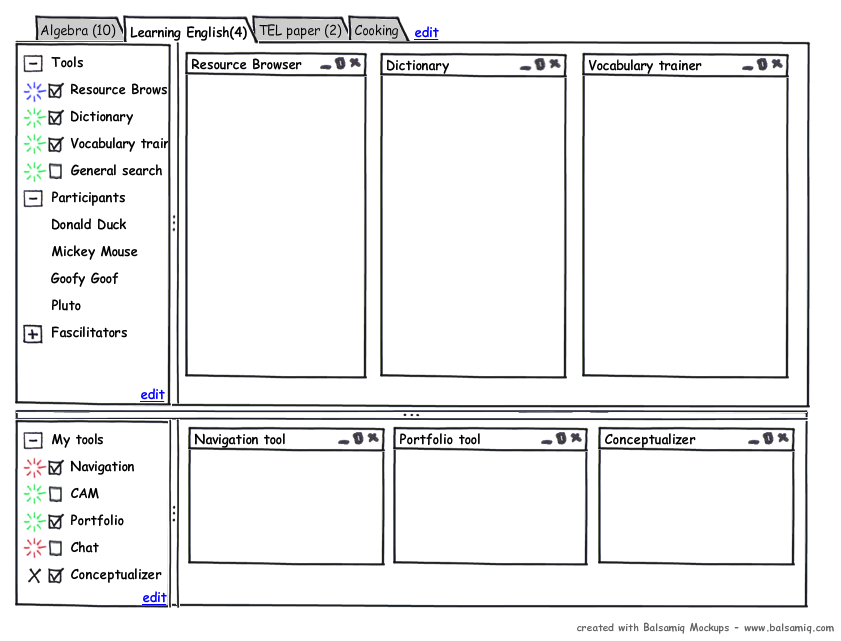
\includegraphics[width=1.0\textwidth] {uu_1.png}
	\caption {First draft from Uppsala Learning Lab}
	\label {fig:uu_1}
\end{figure}

In the first first draft the work space is divided into two areas; one course-related (top) and one personal (bottom). Both areas have a navigation area on the left hand side were tools can be opened or closed by checking or unchecking the box. New widgets can be added and existing widgets can be removed by clicking the edit-link at the bottom of the navigation area. At the top the student can choose which course to work with by changing tab. The student can also create new personal spaces. In this example there is a personal space called Cooking. These personal spaces are not to be confused with the personal area at the bottom part of the screen. On the left hand side you can activate and deactivate the tools for both the personal area and the workspace. Each tool has a coloured icon to the left which shows when widget-communications has been initiated and received. 

\pagebreak
The second version is based on the first sketch but with a few improvements. This version is a working system where widgets can be used to test the concept.
\begin{figure}[h!]
	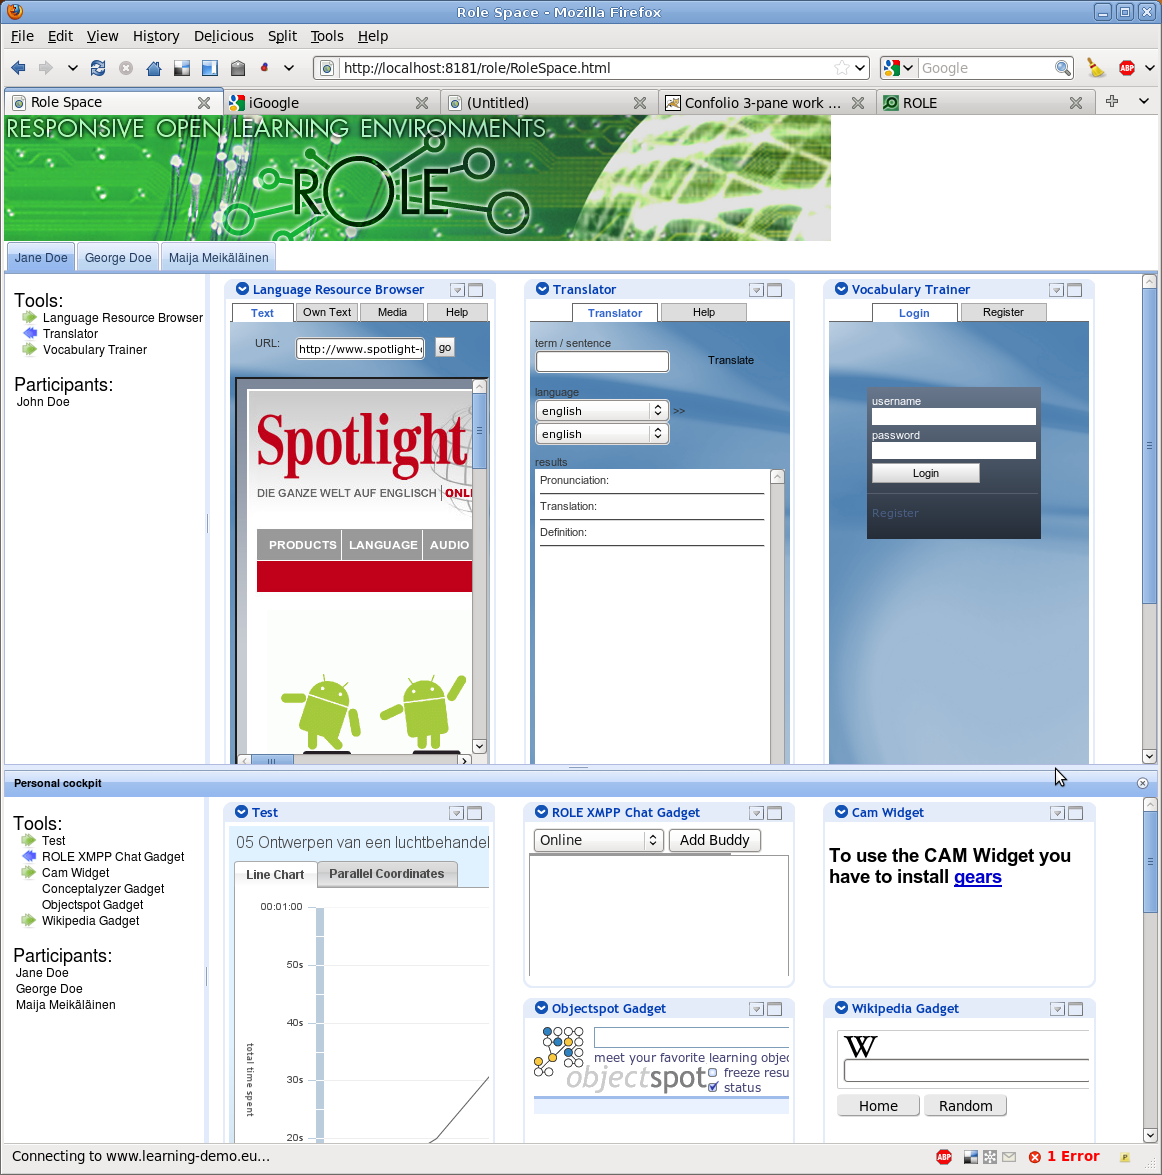
\includegraphics[width=1.0\textwidth] {uu_2.png}
	\caption {Second draft from Uppsala Learning Lab}
	\label {fig:uu_2}
\end{figure}

The major improvement here is in the navigation area on the left hand side. The change of activity icons to arrows clearly shows if an event has been sent or received. The use of shapes, instead of colours only, should help colour blind students. 

\pagebreak
The third version is also a working version. This is an early screen shot of the current version being developed at Uppsala Learning Lab.
\begin{figure}[h!]
	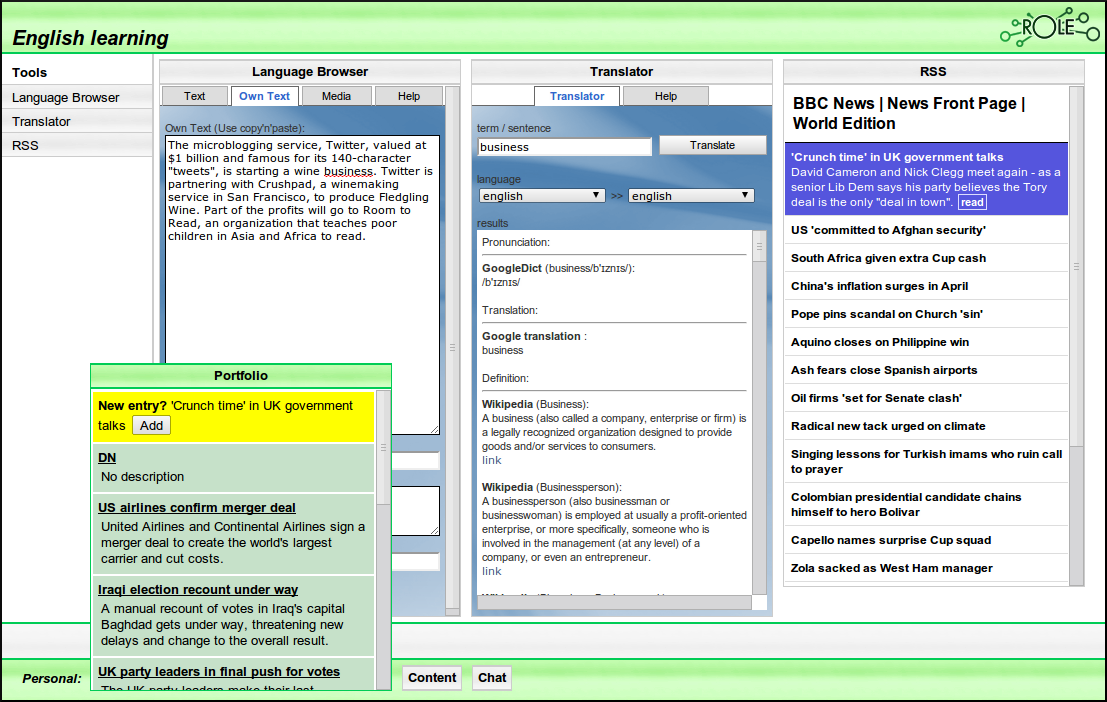
\includegraphics[width=1.0\textwidth] {uu_3.png}
	\caption {Third draft from Uppsala Learning Lab}
	\label {fig:uu_3}
\end{figure}

In this version the personal area has been minimized to a toolbar where the personal widgets will pop up when used. The icons for sending and receiving widget communications have also been removed. The main work area is larger, allowing for either bigger and more readable widgets, or more widgets allowing for easier multitasking. Another change is that different spaces is no longer visible by tabs at the top.

	\section {Requirements}
The major stakeholders in this development project are: The ROLE-project, Uppsala Learning Lab and the users. Requirements from the ROLE-project and Uppsala Learning Lab will be handeled in this section while the user's needs will be taken into account in the next section.

\subsection {Requirements from ROLE}
The ROLE-project has stated the requirements for the entire project. This thesis will only list requirements for a ROLE-based platform, such as PLESpaces (Chatterjee, Law,  Verbert. 2009).

\begin {enumerate}
	\item ROLE should provide users with the ability to construct and maintain a Personal Learning Environment. (PLE)
	\item PLE should support the assembly of learning services / tools / resources.
	\item PLE should allow users to switch between parallel learning context.
	\item Sharing and collaborating in learning contexts.
	\item Data based interoperability of services.
	\item Inter-tool communication in the PLE.
	\item ROLE should support the user in transitioning between different learning situations separated by time or organizational barriers / learning contexts. 
	\item ROLE architecture needs to be appealing.
\end {enumerate}

\subsection {Requirements from Uppsala Learning Lab}
The requirements from Uppsala Learning Lab are mainly interpretations and specifications of the requirements from the ROLE-project. There are, however, some additions: One focus area at Uppsala Learning Lab is the idea of separating different courses into specific “spaces”. These spaces are areas where widgets can be added.

\begin {enumerate}
	\item The PLE should consist of widgets.
	\item Widgets should be able to communicate with other widgets.
	\item Each course should have its own widget space in the students' widget area.
	\item Every student should have a personal space along with the course-specific spaces.
	\item Students should be able to create new widget spaces which can be shared with other students.
\end {enumerate}

	\section {Interaction Design}
During the ROLE-project many sketches have been developed by different contributors. These contributors include, but is not limited to, Uppsala Learning Lab. This section will start by analysing the sketches presented in the previous work section (section 2.5.1). The information gathered from the analysis will be used together with the results from the personas to create new design sketches.

In the ROLE-project most designs are quite similar. This thesis focuses on the designs made by Uppsala Learning Lab as they requested the evaluations.

\subsection {Analysis  of Previous Designs}
The analyses in this section are my personal reflections made with the aid of the ten rules of heuristics listed in the previous work section (section 2.5).

Looking at the sketches made earlier by Uppsala Learning Lab it is clear that a certain concept is being followed. Each course is supposed to have a separate workspace to which widgets can be attached. These tools does not appear in other spaces, and these widgets can not communicate with other widgets outside of the current workspace. This could become a problem if information is to be transferred from one course to another. The solution is a personal widget area which is available on each workspace. This area follows the user to all of his or her workspaces.

In the first version one could argue that the personal area takes too much space. Not allowing the widgets in the workspace enough room. In the second version this is clearly visible. The only reason the image looks somewhat usable is because it is not formatted to a computer screen. When viewing the design on a regular (4:3) monitor the workspace is either be empty on the right or left side or the user would have to scroll down to access the personal area. This effect is even more apparent when viewing on a wide-screen (16:9) monitor. This issue has been addressed in the third version. Here the personal area has been modified into a personal toolbar instead, allowing either more widgets or bigger widgets.

In the first and second version there are indicators next to the widget names on the navigation bars. These are supposed to show the user when widget communications are initiated and received. In the first version these are marked by coloured icons. There are two problems with these icons: The first problem is that the icons take no consideration of the colour blind who may not be able to distinguish between two actions. The other problems is that it is not certain whether these icons are needed in the first place.  This creates a conflict with the first and fifth rule of heuristics. One saying that no extra information should be shown as it may cause confusion and the other saying that the user should always be given feedback on what is going on inside the program. The first problem has been addressed in the second version where arrows have replaced the icons to indicate the direction of the communications. The icons and arrows have been removed in the third design removing the possibility of icons confusing students. Feedback is given by marking new events inside a widget with a new colour and contrast. It is unclear from the sketch if this would be visible if the widget is minimized.

Looking at the first version widgets are opened and minimized using check boxes. This may not be an obvious way to everyone at a first glance but users should not need more than one demonstration to remember it. One issue is that check boxes are not always that easy to click. It should therefore be possible to check and uncheck the box and open widgets by clicking the widget name as well as the check box. In the second and third version these check boxes are not present. According to the people at Uppsala Learning Lab this is not intentional, it has simply not been added yet. The same goes for the ability to add widgets which in the first sketch is done by clicking “edit” in the navigation area. It is very important that this feature is done correctly and in an obvious way since the whole concept of the widget based system is that students are able to find and add widgets that suit them best.

Summarizing the three versions there are some ideas to reuse and some to add.
\begin {itemize}
	\item Divide the working space into a course-specific area and one personal area.
	\item The personal area should not take too much space. A toolbar is one way of doing this.
	\item Adding and removing widgets should be easy to do.
	\item How to open and minimize/close widgets should be obvious.
	\item Widget communications should be visible, but should not interfere with the user's focus.
\end {itemize}

\subsection {New Design Sketches}
These sketches are derived from the sketches made by Uppsala Learning Lab with the ideas from the end of the last section implemented. The sketches are made with the free version of the commercial tool balsamiq. 
The main idea is to have the widget area as large as possible. The widgets should then place themselves inside the widget area when opened. Widgets are never closed, they are just minimized and the information should be available the next time the widget is opened. The widgets are managed by a navigation bar on the side where other resources as fellow students and teachers can be found. At the bottom there is a bar containing the personal widgets.

There are two types of spaces, one is a course space. This space is created by the teacher with a copy distributed to all students. The students will receive the copy at the start of the course. This space will contain widgets recommended by the teacher. The students now have the option to add his or her own favourite widgets in order to make the widget area personally optimized. The other type of space is an empty space where students can create their own space from an empty template. If a student finds his or her space very useful it is possible to share copies of the space to fellow students and also invite fellow students to the space for group assignments and other group activities.

\pagebreak
\begin{figure}[h]
	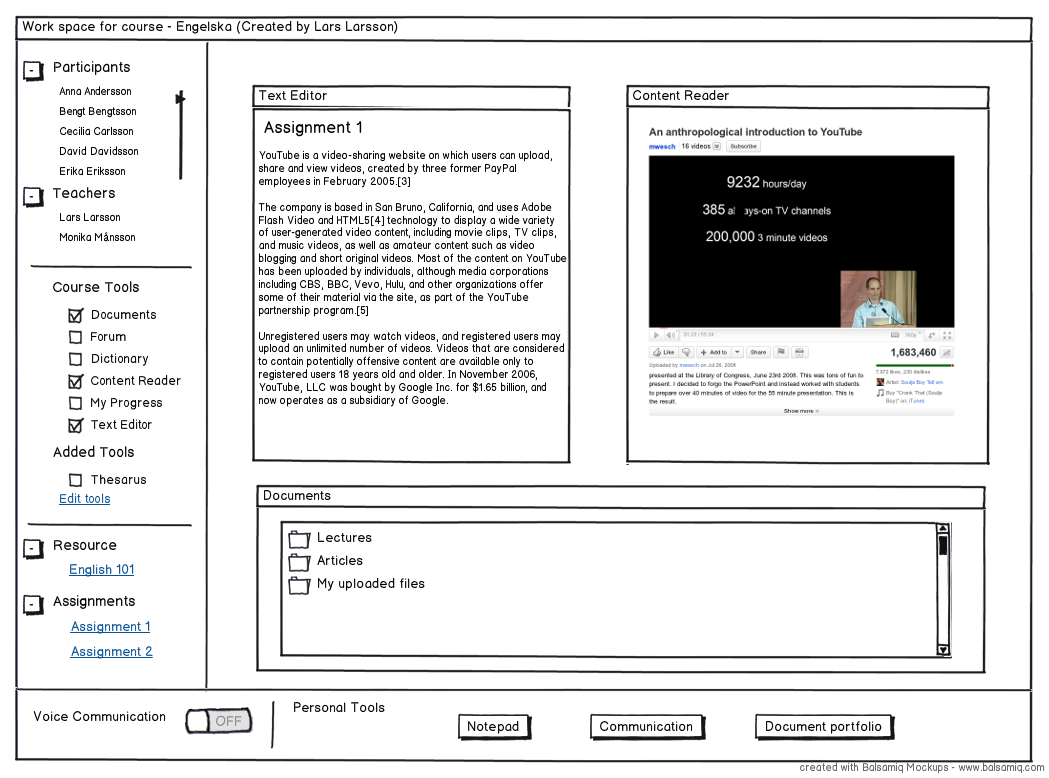
\includegraphics[width=1.0\textwidth] {mj_course.png}
	\caption {Concept sketch of a widget space for a course}
	\label {fig:mj_course.png}
\end{figure}

In the course version the teachers have selected some recommended widgets as a basic version. The student then has the option to add a widget by clicking the link “Edit tools”. The tools added in this design are quite self-explanatory which could be useful when separating a large system into widgets. There is however one widget that may not be so intuitive just by looking at the name. The content reader is a widget that displays contextual information. If a link is clicked in another widget the content reader will fetch the information from that link. If, for example, a YouTube link is visited the content reader will extract the video from the site and only show that instead of displaying the whole page.

\pagebreak
\begin{figure}[h]
	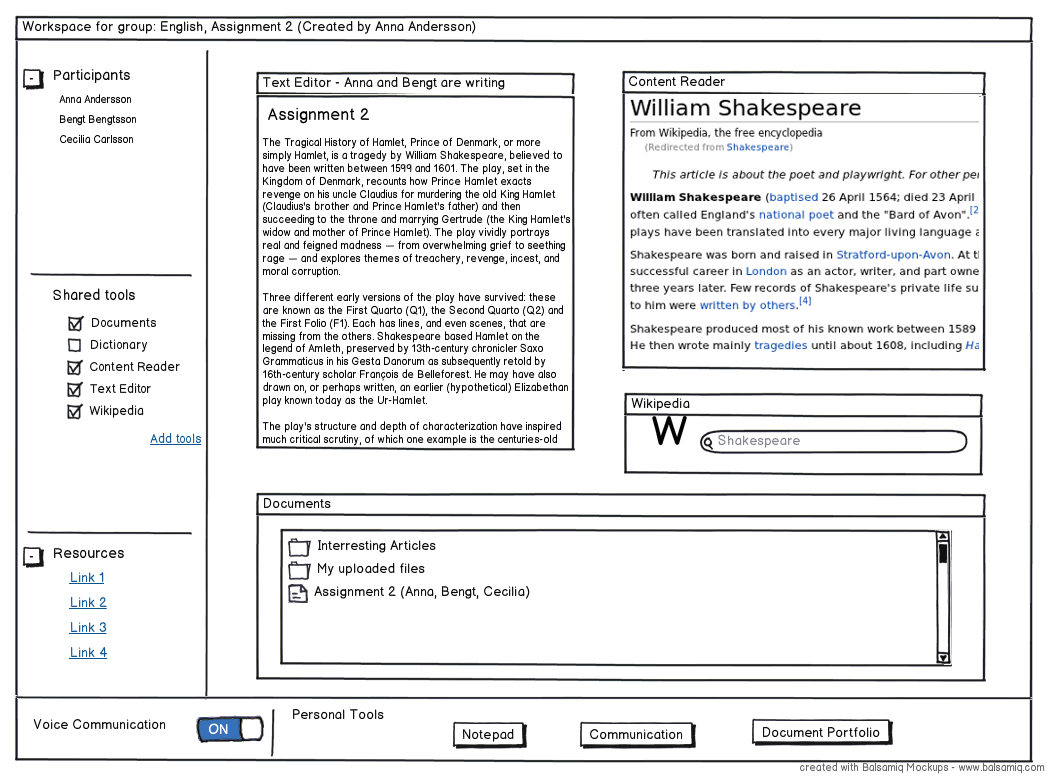
\includegraphics[width=1.0\textwidth] {mj_group.png}
	\caption {Concept sketch of a widget space for a group}
	\label {fig:mj_course.png}
\end{figure}

The empty space version is here implemented as a group version. A student has created a new work space and shared it with two fellow students for an assignment. Together they add widgets they find useful and write their assignment in the collaborative text editor. The functionality of the content reader is visible here. After a search in the Wikipedia-widget the content browser will fetch the requested article from Wikipedia and display it. 

The personal toolbar is the same in both versions to show that it is independent from the current work space and is the same everywhere in the system. The personal toolbar will have to be edited in a special screen. This could be done from a personal menu screen where other personal settings are edited and where workspaces are managed.

	\section {Usability Recommendations}
The ROLE-project finds four typical user groups: Users, peers, tutors and teachers. \cite{chatterjee} This thesis will focus on students. This is mainly since there is not enough time to investigate all users. Students are chosen because they are the, by far, largest user group and also because the author of this thesis is a student.

At Uppsala University there are many different courses where students and teachers have different needs and different tools available. In most basic courses the student groups can be large with more than a hundred students attending lectures and writing exams together. Some advanced courses only have 20-30 students in class, allowing the teacher to have a more personal relation to the students. There are also distance courses where the teacher may not even see the students once. Students and teachers in these courses have different needs which must be reflected upon and taken into account when designing a new system.

\subsection {Personas}
This thesis will use personas to represent different user groups. The personas will be presented in the first section. In the second section a scenario will be presented and in the third section the personas will be used in the scenario to find recommendations based on different user groups.

\begin{wrapfigure}{l}{0.2\textwidth}
  \begin{center}
    
\includegraphics[width=0.18\textwidth]{Mikael.png}
  \end{center}
\end{wrapfigure}
\textbf {Mikael:} Mikael is 30 years old. Mikael is taking a course in Swedish. He has earlier worked at a film distribution company. After a few years of work he has again found his passion for languages and is now studying to become a translator, hoping to combine his interests in films and languages. Mikael lives with his girlfriend and their 2 year-old daughter. Mikael's girlfriend wants to get married, but Mikael wants to finish his studies and get his career going before planning a wedding.
At the university Mikael is doing fine. He plans his studies and makes sure he has reads everything thoroughly in time for examinations and seminars. He often takes responsibility and sets up sessions for him and his friends to study together.
Mikael is not really a computer guy. He uses his computer to read the news and to update facebook from time to time. But mostly he visits different forums to discuss films in different genres. The favourite genre is Japanese animé. A few years back Mikael spent some time in Japan to get acquainted with the Japanese culture and language. After all the writing on forums and watching foreign films Mikael consider himself to be very proficient in English. His goal is therefore to become a translator for Japanese and English films.

\begin{wrapfigure}{l}{0.2\textwidth}
  \begin{center}
    
\includegraphics[width=0.18\textwidth]{Therese.png}
  \end{center}
\end{wrapfigure}
\textbf {Therese:} Therese is 23 years old. She is currently studying the candidate programme in economics. Therese has a fondness for fashion and spends a lot of time visiting and writing blog posts regarding fashion. This led to her getting a job as a salesperson in a fashion store after graduating from high school. Two years later she started her studies at the university. She really liked her work but she felt the fashion business really did not offer a future for her as she did not have a higher education, and designing was not really her calling. Therese is hoping to get a job as a business administrator at a fashion company. 
Therese lives in a student dorm with 5 others and she really likes the social aspect. The only down-side is that the kitchen is always messy. She would take more responsibility to organize cleaning in the dorm, but it is currently managed by one who has lived there longer and the rest does not seem to mind the messy kitchen. 
To stay in shape Therese goes to the gym for spinning and in the summer time she takes long jogging sessions with her favourite music loaded on her iPod. Therese's studies are no problems, the only problem is all the parties going on. As she is active in one of the student nations her social schedule is quite busy with her dorm mates, people from school and also the active people at the nation.

\begin{wrapfigure}{l}{0.2\textwidth}
  \begin{center}
    
\includegraphics[width=0.18\textwidth]{Benjamin.png}
  \end{center}
\end{wrapfigure}
\textbf {Benjamin:} Benjamin is 20 years old. After finishing high school he went directly to the university to start a bachelor programme in computer sciences. Ever since his family got their first computer when Benjamin was 5 years old he has been fascinated by computers and computer games. In high school he took a few programming courses, but mostly he learned by himself. It started when Benjamin played computer games and his team needed a website. Benjamin took the opportunity to learn web coding and then moved on to more traditional software development.
Benjamin lives in a student dorm with 11 other people. He likes the people living there but he does not spend that much time with them. He spends most of his free time with his classmates, playing retro computer games.
Computer science studies are quite individual in the beginning which fits Benjamin perfectly. Benjamin does not have a problem with teamwork, he just prefers working by himself and setting up his work in his way. Benjamin's future is not really planned out. He is satisfied with where he is right now and tries to enjoy his studies and everything around it while it lasts. What he will do for real when his studies are finished will have to wait until later.

\subsubsection {Scenario}
The university where Mikael, Therese and Benjamin are studying has a web based IT-system where all courses are managed. Each course has its own web space where teachers can upload information and assignments and where students can upload solutions to the assignments. The three courses that Mikael Therese and Benjamin are taking have been selected for testing the new widget based personal learning environment. This system is based purely on the idea of the psycho-pedagogical integration model. The system is not an implementation of the PLESpaces software.

During the course the students will be given an empty workspace where they are supposed to add widgets they feel useful. They will receive one individual assignment each to finish by using the widgets they added. After the individual assignment they will be given one group assignment each to finish within their groups which will contain random classmates.

\textbf{Mikael} As Mikael is not really a computer guy he has never used any previous system based on widgets. This means that he does not grasp the concept of having small tools that all work independently. Instead he sees the whole workspace as one program that currently does nothing. After a couple of days of trying to understand what the system is about he has managed to add a word processing widget and a widget for finding academic articles. This work has taken much time and Mikael now has to focus on his assignment. Since he is feeling a bit stressed he goes back to his old way of studying, meaning he searches for material in his usual way and writes his assignment in his standard word processor and in the end copies it into the word processing widget and hands it in. The assignment made Mikael quite annoyed, the system just does not work as he expects it to.

For the group assignment he is lucky that someone else in the group has managed to learn a bit more of the system and creates a shared workspace for the group. Mikael is however not alone to have had problems with the individual assignment and there is some resistance against using the new system. In the end the group decides to use the word processing widget for concurrent writing and a shared notepad for writing notes and adding references. For communication the group uses Skype and e-mail.

\textbf {Therese} Therese on the other hand is somewhat used to computers. For the individual assignment she is quick to set up a word processing widget and one widget for spreadsheets. However, since she has never used the system earlier her major problem is that she has no idea what kind of widgets are available. Are there widgets for seeing interest rates in US for the last five years, and what are they called? There are tips in the forums but as Therese has not added the forum widget, in fact she does not even know there is such a widget, so she does not see the them. In the end she has to rely on the tools she usually uses to finish the assignment.

For the group assignment her groups is rather mixed. Some managed to find the forum and read the tips where others never even used the system since they had no understanding of it. Due to time constraints the group work is divided where the members who did not use the IT-system are assigned to find data that can not be found with the current available widgets where the rest, including Therese, use the IT-system to analyse the data and write the report. Since not all of the members are using the system to do their work they are not available for the communication which takes place inside the system.

\textbf {Benjamin} Benjamin's individual assignment is a programming assignment. He is supposed to develop part of program. Students do different parts which each perform a specific task. He starts by looking through the available widgets and finds the widgets for the forum and the one for reading course-related material. He reads through the lecture notes and the assignment specifics. He now has an idea how to finish his assignment, but he needs some more help. Usually he just searches the web for help, so he adds a widget for displaying search results and saves all the links he needs. Lastly he adds a widget for writing code and starts his coding assignment. After a while he realizes that he needs the code on his own computer to compile the program, so he transfers all his code to his own computer and finishes the assignment there, using the IT system as a source for information.

The group assignment is to take the different parts from the individual assignment and merge them together into a whole program. One of the group members takes command and sets up a shared workspace with communication, a widget for reviewing the code all the group members made and a widget for writing the code together. Benjamin is happy that someone else takes command, but is not happy with the way the workspace is set up. He changes the workspace but it changes for everyone else which causes some argument in the group. In the end the group leader again sets up the workspace and tells everyone else to be happy with the layout, or at least stop arguing about it.

\subsubsection {Results from personas}
After looking through the scenario and the personas' problems and success a few concerns arise. These must be taken into account when designing a new IT system like PLESpaces. These will, along with results from the survey be discussed in the analysis and discussion sections.
\begin {itemize}
	\item The concept of widgets and the widget communication may not be clear to everyone.
	\item Users must see a clear advantage of using the IT system instead of their usual tools.
	\item Finding and adding widgets may take focus away from the actual assignment.
	\item Specific widgets must be easy to find and add.
	\item If communication is to take place inside the IT system everyone must have access to it.
	\item Some tasks may not be able to be performed within the IT system.
	\item Shared workspaces may cause confusion if everyone can change it.
\end {itemize}

\subsection {Survey}
A survey was handed out to the students in the course Social Media and Web 2.0 at Uppsala University. The course is a distance course so the surveys could not be handed out personally. Instead it was managed through a free online survey service called Kwiksurveys. To encourage students to fill in the survey a gift card for the cinemas was sent to everyone who finished it. In the end 21 out of 34 students sent in their answers.

The complete survey and results can be found in the appendix (section A). This section will report on the important findings.

The survey starts out by asking a few personal questions, such as age, gender and how long they have been studying. The results show a slight majority of men (57\%) and an average age of 25 with the oldest at 38 and the youngest at 21. The experience from university studies is quite high where everyone has studied at least one year and almost half (48\%) with more than three years of studies.

The survey continues to investigate what the students think of the current IT system, called Ping Pong. The results from the survey shows that the system is easy to navigate (62\% vs 10\%, meaning 62\% agree or strongly agree and 10\% disagree or strongly disagree) but does not allow students to adapt it to their needs (52\% vs 14\%).

The next part concerns how the students study today, in order to adapt a new system like PLESpaces to their needs. The first question regards communications, and it has to be remembered here that the course is a distance course which may affect the answers. The results show that students are no strangers to using a built-in solution, 52\% say they use it often or very often. This can be compared to the other communication options, e-mail (28\%), telephone (10\%) and third party clients, like MSN or Skype (5\%). 
The survey continues by investigating how students study at the computer. When asked if the students are used to multitasking in a IT-environment. 89\% say they often have multiple windows open at the same time when studying. It also finds that 71\% often or very often use the computer to find relevant academic articles and 86\% often or very often use it to find free material (such as Wikipedia articles). Only 20\% often or very often visit the library to find relevant material.

Students are now shown the design sketch from the previous section (section 4.2) and asked for their opinions about it. This sketch is also meant to show the concept of widget based systems.
81\% consider the design to be easy to navigate. 71\% think the design would be easy to use.
This is followed by questions regarding the concept of widget based systems. Students are now asked what they think of widgets communicating with each other. The question asks if this would be assisting or hindering the student's studies. 67\% think it would be helpful and 5\% think it would hinder them. At the bottom of the design there is an area with personal widgets. When asked if the students would use this 62\% said yes and 24\% said no. Regarding the concept of widget based systems 62\% believe a system built on widgets could be made to be at least as easy to use as today's systems. It should also be noted that only 24\% had previous experience in using systems based on widgets.

The survey now moves onto questions specifically asked by ROLE or Uppsala Learning Lab. The first questions asks if the student would prefer to build a widget space from scratch for a course or if the teacher should provide a basic version. 90\% said they would prefer a system suggested by the teacher. Other questions regard the concept of setting up goals for a course. The first questions is who should set up the goals. 57\% say the teacher should set up goals together with the student, 24\% wants the teacher to set up the goals and 19\% would like the teacher to suggest goal from which the student choose his or her personal goals. Notably 0\% wanted to create their own goals.
67\% wants the creator of the goal to decide if the goal is achieved, 10\% say the student should decide and 14\% say the teacher. It should be noted here that students were mostly consistent. Those who wanted the teacher to set the goals also wanted the teacher to decide (or the creator, which in that case would be the teacher). There was one exception, one student wanted the teacher to set the goals but he or she wanted to decide if they were achieved by him/herself.
When asked if the teacher should be allowed to see the goals 62\% said yes, 24\% said the teacher may see the goals, but not if they have been achieved or not. There were no students saying the teacher could not see the goals.
The last questions asks if the student would like to receive recommendations from the system. These recommendations would be based on the goals set. 81\% said they would like recommendations of widgets that could help them in their studies. The same amount would like recommendations of articles or web-based material that could aid them in their studies. 67\% said they would like recommendations of new goals and subgoals. The same amount would also like recommendations of fellow students to cooperate with.
Even though the same amount of students answered yes on the first two, and another amount answered yes on the other two it was not the same students.

\subsubsection {Results from the survey}
The sample group contains an almost equal amount of men and women. The age span is from 21 to 38 where 25 is the mean value. The results could therefore be seen as representative of the students at Uppsala University.

\begin {itemize}
	\item The current system is easy to navigate but does not allow students to personalize it.
	\item Students have no problems using a built-in communication system.
	\item Multitasking and having multiple things on the screen at one time is nothing new.
	\item Students use the computer as their main source to find relevant sources.
	\item Widget communication would probably be a helpful concept.
	\item The concept of widgets would not be difficult to learn.
	\item A personal toolbar would be useful.
	\item A big majority would like to receive a recommended set up for the workspace.
	\item None of the students wants to create his or her goals. Instead the teacher should create them together with the student.
	\item Most students have no problems with teachers seeing their set goals.
	\item Automatic recommendations from the system is a good thing
\end {itemize}

	\section {Analysis}
This section will summarize the answers to the questions stated in the introduction (section 1) and some thoughts about them. This section will be a bit more personal than the earlier parts of the thesis as it will reflect the author's interpretations of the results.

The purpose and goal for this thesis were to:
\begin {itemize}
	\item Investigate how the psycho-pedagogical integration model can be implemented in PLESpaces in the way intended by the ROLE-project.
	\item Look at current prototypes and use them to create interaction design sketches for PLESpaces
	\item List usability recommendations for PLESpaces
\end {itemize}

\subsection {Integrating PPIM in PLESpaces}
As stated in the previous work-section (section 2.3) the psycho-pedagogical integration model divides learning into four phases. In the first phase the student is supposed to set up his or her goals for learning. No feedback regarding this is given from personas, but the real life students answering the survey delivered valuable input. Not one of the students answering the survey wanted to create his or her own goals. Instead the teacher should create goals together with the student. This may not be that realistic, specially in large courses. The ability to create goals can be integrated into PLESpaces, but I seriously doubt the possibility would be used by today's students. If we now assume that students will not create their own goals they will probably only use the system to reach the courses' goals, such as assignments. So PLESpaces will in this case be a personal learning environment without focus on the students creating their own goals. One could argue that students already set up sub goals based on the assignments set by the teacher. This is simply a method of problem solving where the main task is divided into subtasks. As a personal reflection I have only taken one course at the university where special emphasis was given to setting up personal goals and following up on them. This course was a 15 credit project course with 22 students and 3 teachers. I doubt this would have worked in a 10 credit math course with 200 students and 5-6 teachers.

In the second phase of PPIM the student is supposed to find tools to reach the goals set in phase one. In the ROLE-project this translates to adding specific widgets to the student's workspaces. Continuing from the analysis of phase one, where students do not create their own goals, students would now add widgets that will help them to solve goals set by the teacher, such as assignments. The information from personas suggest that finding these tools may take focus from solving the actual assignment. Responses in the survey suggest that students want a basic version prepared by the teacher instead of creating their workspace from scratch. This is not that surprising. It is rare, at least in courses I have personally taken that students are expected to find course material on their own. It does happen that we are supposed to find an academic article about something and refer to it. But the basic material is often prepared by the teacher. Again, as a personal reflection I have only been assigned to find material by myself in one or two courses, not counting this thesis.

The third phase regards working with the selected tools to reach the set goals. This phase should be no problem to integrate in PLESpaces as long as the interface is usable. The main issue would be to make students use it in the first place instead of using their own set up with OpenOffice, Firefox, Skype Google Calendar and Hotmail.

The fourth phase is aimed at reflecting on the learning and how well problems were solved. Personally I have rarely done this, at least not consciously. I have noticed that I use my favourite places to find the information I need, but I rarely have the time to actively reflect on what was good and what wasn't after finishing an assignment. The thesis does not give that much feedback on how this could be implemented. As most courses are today I make sure to finish the last assignment by the last day of the course and then I start a new course the next day. Even with an IT-system with support for this there is just no room for these reflections. The one thing that comes to mind is the reuse of tools. If a tool is used in one course and found usable it will likely be used again in later courses and hopefully recommended to other students. This could be seen as a reflection but it would not be a separate phase rather than a merge between phase three and four.

To summarize: PPIM can partially be implemented. The first phase will be difficult. Creating basic goals like assignments will, just as today, make students create sub goals to finish the main goal. The most realistic method would be to encourage students to use a task manager where they list what they need to do. Whether this can be interpreted as setting up goals is something that can be discussed further. The second phase can be partially integrated. I believe it will be very difficult to make students build their environments from scratch. Instead teachers should provide a set of basic workspace to which students can add their own favourite widgets if needed. The third phase should be able to be integrated without problems and the fourth could perhaps be merged into phase three.

\subsection {Design Sketches}

To create the design sketches presented in this thesis I took the most usable parts from the existing sketches and rearranged the workspace to reflect the results I found in my analysis of those sketches. The new sketches are designed for students used to how websites look today. The new designs were presented to the students filling in the survey and the feedback was positive. A big majority thought the system would be easy to use and navigate. Since the work inside the ROLE-project is not finished I doubt the final version will look like this as new features have to be added when new discoveries are made within the project. However, I do believe that some elements in this design will be quite usable in the final design.

\subsection {Usability Recommendations}
The list of recommendations I came up with can be found in the section with the same name (section 5). Here I will just list the most important ones and explain why I find them important.

“Users must see a clear advantage of using the IT system instead of their usual tools.” (section 5.1) - Everyone works differently, we all have our own personal way of solving problems. Some are more effective than others but it is not often possible to say that one way is better than another. This is reflected in the way students work in school as well. When I've taken a look around the classroom during assignments all screens have been different. Information sources are different, the way of writing code is different and the screens show different programs and windows. It will not be easy to convince students that this new system will be better than the system they have set up in their own way at home. It might be a good idea to focus on the social aspects, like communication and cooperation.

“If communication is to take place inside the IT system everyone must have access to it.” (section 5.1) - Communication is arguably one of the most important aspects of team work and needs to be accessible for everyone. I would suggest that direct communication should be kept in the personal area. Having it in the personal area makes sure it is always present. The only issue might be that communication from other courses may interrupt the students work. One way of solving this is to set availability on a course level, so only people in the active workspace can see that the student is online. A widget for forum and general communication within a workspace should not be possible to remove, only minimized.

“Students use the computer as their main source to find relevant sources” (section 5.2) - I think Uppsala Learning Lab should focus on this. If PLESpaces can be used to effectively find sources like articles and books or just to check some fact, like Wikipedia and WolframAlpha, students may find it very useful. Using that feature might be an entry to other widgets as well.

“Automatic recommendations from the system is a good thing” (section 5.2) - It seems students would like to receive recommendations. The most requested recommendations were widgets that might help do their work more efficiently or find relevant sources in a specific subject. From a usability perspective I would suggest that these recommendations are very subtle. I personally find it quite annoying when a program is trying to tell me something that I haven't requested. I'm not sure whether these recommendations should be able to be turned off. I would personally turn them off in one second since the “tip-of-the-day” dialogues in many programs just aren't helpful. These recommendations might be seen as the same thing.

\subsection {Analysis of the Survey Results}
Most of the answers were in line with my personal oppinion as a student at Uppsala university. There were some differences and other notable results I would like to discuss here:

62\% think Ping Pong is easy to navigate: Personally I would have clicked disagree or strongly disagree. This may be becuase I am more used to computers than others so I expect software to be designed and  behave in a certain way. In any case I have found myself clicking every single link in Ping Pong just to find where my teacher uploaded the assignment I am supposed to do.

When asking students what they think of widget communication 5\% answer they think this feature would hinder them. Even though it is very difficult to make a system that everyone will like I find it hard to get the reason for this response. My best guess would be that those who answered that it would hinder them are either not that used to computers or did not really reflect on what the text meant. I believe that the reason behind Microsoft's success is that all programs delivered with the operating system Windows and the office suite Office are very well integrated and communicate with eachother. However, when designing a system with widget communication you could reduce the confusion for users by making sure the user stays in control.



	\chapter{Discussion}

\setcounter{section}{7}
\setcounter{subsection}{0}

\subsection{Test-driven development in Javascript}

Test-driven development is something that is not used very much today by Javascript developers. If a framework can provide an architecture that helps developers to get around the problem with writing simple unit tests it will most probably be used more than it is today. As seen in the thesis it is possible to achieve high degree of testability if just the testing aspect of the application is considered already in the design phase of the system.

\subsection{The importance of delays}

The initial loading time has been considered as an important aspect of SPAs in the thesis since it directly affects the users. If the users are not satisfied the website will become less popular. However, another study suggests that the time it takes to interact with the website is even more important than the initial loading time \cite{user_interactivity_tolerance}. Users were asked to rate the quality of a service when the delay was varying. The result showed that the tolerance for delay is decreasing over time. Users were more patient the first time the page loaded than when interacting with it later on. This explains why SPAs are so popular, they have a slow initial loading time but that is also when the users are as most patient. It also highlights why SPAs are well suited for websites with a high degree of user interactivity. SPAs perform well after the page has loaded which corresponds to when the patience is decreased.

\subsection{When to use SPAs}

As explained above SPAs are great for all websites that involve a high degree of user interactivity, like websites that are more like applications rather than traditional web pages. They are also great to use for websites that target mobile devices. In some cases SPAs are even considered as an alternative to native mobile applications. If a mobile application is written as a web application there is only one version to maintain. If instead a native application would be developed there would be one version for each operating system. It would of course result in both higher development and maintenance costs. On the other hand the user experience will be a lot better in a native application since it always will be able to perform better than a web application. 

For websites that are dependent on very precise SEO SPAs are most probably not such a good choice. Unless the crawlers start to execute Javascript will a separate solution for SEO always be needed. All these solutions have their limitations, a traditional website does not. Today it is often hard to get tools for web analytics to coop with SPAs, these tools are essential to develop a good SEO strategy. The problem is that since a SPA never reloads the page the user actions will not be posted to the analytics tool, which results in the visitor flow not being analyzed. Another problem with SPAs is that users with accessibility tools, such as screen readers, might have a hard time using the application. Most of these tools have a limited support for websites that asynchronously changes its content, which of course will make SPAs hard to use.

% A well thought-through system design is really helping to get better maintainability. Think of dependencies etc.
% Using configurable dependencies makes the framework both flexible and smaller

\subsection{Future work}

An interesting question to ask if whether MinimaJS is a realistic alternative to existing frameworks on the market. The framework is of course in an early development phase and more testing is needed before using it in production. Especially browser compatibility is an important aspect when targeting a wider market, this is an aspect that has not been considered at all during the development. However, there is nothing in MinimaJS that is impossible to implement to support the browsers that are popular today. To get it to work in all major browsers it would probably not require too much work. Documentation is another thing that has to be improved, it is an essential aspect to consider to enable other developers to learn the framework.

Since the framework performed very well in the tests compared to its competitors the future is looking bright. Especially when it comes to testing which is something that is becoming an even more important part of the development.

	\section {Future Work}
These questions are derived from the analysis and the discussion in the previous sections. I would suggest looking into these questions before launching a system like PLESpaces.

\textbf {Interactive Recommendations:} The survey shows that students would like to have contextual  and automatic recommendations inside the system. Students specially requests recommendations as tools to use and where to find reliable sources. This area would need some extra investigation. What kind of recommendations should be shown? When should the recommendations be shown? Should the student be able to turn them off?

\textbf {Making Students use the System:} Today students have their own personal learning environment set up. Making them switch may not be easy, some students may even have paid for commercial program licenses. The students must see a clear advantage in order to change, preferably without being forced into the system. Maybe focus should be on the social aspect of cooperation?

\textbf {Personal Goals:} As it is today students are not very keen on setting their own goals. In fact not a single one in the survey wanted to set their own goals. The questions here is simple: Should the method of setting goals be forced upon the student or not? If yes: How would this be done? If not: Should someone else set up the goals, or should this phase be discarded in the system?

\textbf {Choosing tools:} This phase is not widely accepted. The survey and personas show that students does not want to create their own set up. Instead the teacher should set up a basic version which students can edit at will. Group spaces can be left empty and students build their own workspaces there instead. Is this an acceptable implementation according to the PPIM?

	
	\bibliographystyle{plain}
	\bibliography{references}
	
	\appendix
\section {Survey}
The survey was given in Swedish, this is my translation of the survey to English. The survey was done through a web service called kwiksurveys (www.kwiksurveys.com). 

\textbf{Page 1 - Introduction}

A current EU project called ROLE is currently taking place around Europe. The purpose is to encourage students to take more responsibility for their own learning. One step is to allow students to build their own learning environment.
The main quiestion for ROLE is if this could be done with an IT-system. Uppsala Learning Lab who administrate “Studentportalen” and “Ping Pong” are currently developing an experimental platform to investigate this. Please note that there are no current plans to develop such a platform to replace “Studentportalen” or “Ping Pong”. The project at Uppsala Learning Lab is just an experimental platform developed for research.

This survey aims to get students' feedback regarding the current system used at Uppsala University: Which tools are used? Which tools are not used? Which tools are missing?
At the end of the survey you will find a sketch of what the new experimental platform could look like. Following the sketches are a few questions where you are asked what you think of them and if you would use such a system if it was available.
Page 1 – Who are you?

1. Sex

\begin{center}
    \begin{tabular}{ | l | l | }
    \hline
    Male & 57\% \\ \hline
	Female & 43\% \\ \hline
    \end{tabular}
\end{center}

2. Age - Oldest: 38, Youngest: 21, Average: 25

3. I've studied at a university for:

\begin{center}
    \begin{tabular}{ | l | l | }
    \hline
    < 1 year & 0\% \\ \hline
	1-2 years & 24\% \\ \hline
	2-3 years & 29\% \\ \hline
	3-4 years & 14\% \\ \hline
	4-5 years & 19\% \\ \hline
	> 5 years & 14\% \\ \hline
    \end{tabular}
\end{center}

\textbf{Page 2 - Your thoughts on the current system}
At the following questions you can answer from 1 to 5 where 1 = I do not agree at all and 5 = I fully agree.

4. I see myself as an experienced user of Ping Pong:

\begin{center}
    \begin{tabular}{ | l | l | }
    \hline
    1 & 0\% \\ \hline
	2 & 24\% \\ \hline
	3 & 43\% \\ \hline
	4 & 24\% \\ \hline
	5 & 9\% \\ \hline
    \end{tabular}
\end{center}

5. Ping Pong is easy to navigate:

\begin{center}
    \begin{tabular}{ | l | l | }
    \hline
    1 & 0\% \\ \hline
	2 & 9\% \\ \hline
	3 & 29\% \\ \hline
	4 & 48\% \\ \hline
	5 & 14\% \\ \hline
    \end{tabular}
\end{center}

6. I can modify Ping Pong to better suit my needs:

\begin{center}
    \begin{tabular}{ | l | l | }
    \hline
    1 & 9\% \\ \hline
	2 & 43\% \\ \hline
	3 & 34\% \\ \hline
	4 & 9\% \\ \hline
	5 & 5\% \\ \hline
    \end{tabular}
\end{center}

7. I use all the functions available in Ping Pong

\begin{center}
    \begin{tabular}{ | l | l | }
    \hline
    1 & 9\% \\ \hline
	2 & 67\% \\ \hline
	3 & 19\% \\ \hline
	4 & 5\% \\ \hline
	5 & 0\% \\ \hline
    \end{tabular}
\end{center}

8. I have seen the following tools in Ping Pong (even though I have not used them)

\begin{center}
    \begin{tabular}{ | l | l | }
    \hline
    See my progress & 95\% \\ \hline
	Upload/download documents & 100\% \\ \hline
	Frequently asked questions & 95\% \\ \hline
	List students & 100\% \\ \hline
	Bulletin-board & 66\% \\ \hline
	Discussion forum & 100\% \\ \hline
	Contact the teacher(s) & 76\% \\ \hline
	Private messages & 71\% \\ \hline
	Notes & 33\% \\ \hline
	Calculator & 24\% \\ \hline
	Calendar & 24\% \\ \hline
	Document portfolio & 38\% \\ \hline
	Log book & 5\% \\ \hline
    \end{tabular}
\end{center}

					
9. I have used the following tools in Ping Pong

\begin{center}
    \begin{tabular}{ | l | l | }
    \hline
    See my progress & 95\% \\ \hline
	Upload/download documents & 95\% \\ \hline
	Frequently asked questions & 81\% \\ \hline
	List students & 90\% \\ \hline
	Bulletin-board & 43\% \\ \hline
	Discussion forum & 95\% \\ \hline
	Contact the teacher(s) & 52\% \\ \hline
	Private messages & 38\% \\ \hline
	Notes & 5\% \\ \hline
	Calculator & 14\% \\ \hline
	Calendar & 0\% \\ \hline
	Document portfolio & 24\% \\ \hline
	Log book & 0\% \\ \hline
    \end{tabular}
\end{center}

10. Is there any tool you are missing in Ping Pong?


	"Access to material from earlier editions of the course - Students are too limited to the material uploaded by the teacher" \\
	"Having the mail at the same place" \\
	"Possibly some form of simplification and more distinct tabs" \\
	"There should be some sort of time plan (date and task), which are filled as you progress" \\
	"A feed that is constantly present, and in such a way that the feeling of activity is boosted." \\

\textbf {Page 3 – Your learning methods}
Here are some questions regarding your learning methods. You answer on a scale from 1 to 5 where 1 = never and 5 = very often. In some questions you may click “other” and add your own ideas.

11. To communicate with my classmates I use:

\begin{center}
    \begin{tabular}{ | l | l | l | l | l | l |}
    \hline
    Option & 1 & 2 & 3 & 4 & 5 \\ \hline
	Communications inside Ping Pong & 29\% & 5\% & 14\% & 14\% & 38\% \\ \hline
	E-mail & 62\% & 5\% & 5\% & 14\% & 14\% \\ \hline
	Third-party system (MSN, Skype etc) & 62\% & 14\% & 19\% & 5\% & 0\%\\ \hline
	Phone & 67\% & 10\% & 14\% & 0\% & 10\% \\ \hline
	Other & 95\%& 0\% & 0\% & 0\% & 5\% \\ \hline
    \end{tabular}
    Other: Facebook groups.
\end{center}

12. When we are writing a group assignment we:

\begin{center}
    \begin{tabular}{ | p{8cm} | l | l | l | l | l |}
    \hline
    Option & 1 & 2 & 3 & 4 & 5 \\ \hline
	We meet in school or at another physical location & 48\% & 5\% & 5\% & 33\% & 10\% \\ \hline
	We split the task/document into parts and all group members do their part & 29\% & 19\% & 19\% & 14\% & 19\% \\ \hline
	We work in the same document at the same time (e.g. Google Docs) & 48\% & 14\% & 19\% & 14\% & 5\%\\ \hline
	Other & 81\%& 0\% & 5\% & 0\% & 14\% \\ \hline
    \end{tabular}
    Other: Dropbox, Built-in forum.
\end{center}

13. When I work with my own tasks:

\begin{center}
    \begin{tabular}{ | l | l | l | l | l | l |}
    \hline
    Option & 1 & 2 & 3 & 4 & 5 \\ \hline
	I only have one window open. & 90\% & 10\% & 0\% & 0\% & 0\% \\ \hline
	I frequently switch between a few windows. & 29\% & 19\% & 29\% & 10\% & 14\% \\ \hline
	I have a lot of  windows open at the same time. & 5\% & 0\% & 5\% & 19\% & 71\%\\ \hline
    \end{tabular}
\end{center}
	
14. When searching for study material:

\begin{center}
    \begin{tabular}{ | p{8cm} | l | l | l | l | l |}
    \hline
    Option & 1 & 2 & 3 & 4 & 5 \\ \hline
	I visit the library & 43\% & 24\% & 14\% & 10\% & 10\% \\ \hline
	I search for academic articles on the web (Uppsala University's “Samsök”, Google scholar etc). & 5\% & 5\% & 19\% & 19\% & 52\% \\ \hline
	I use free services to search for material (Google, Wikipedia etc) & 5\% & 10\% & 10\% & 24\% & 52\%\\ \hline
	Other & 95\%& 5\% & 0\% & 0\% & 0\% \\ \hline
    \end{tabular}
    Other: Dropbox, Built-in forum.
\end{center}

\textbf {Page 4 – A layout draft for the new experimental platform}

(Students are now shown the images available in the Interaction Design section.)

These images are just a draft of what the system could look like. The imortant part is not the design in itself but the underlying concept.
Look at the images and then answer a few questions using the same pattern as before (1=I do not agree at all, 5 = I totally agree).

The concept is to use a more flexible system than the ones used at Uppsala University today. This should allow the student to create his or her own learning environment.

The platform makes use of small tools (called widgets) which has specific uses. This could be anything from uploading/downloading files, to word processors and communication tools.
Every course has its own space where tools can be added. The course-specific space is created by the teacher. The teacher also add tools that could help the students. Students are then able to add and remove widgets by themselves to create a more personal learning environment. At the bottom you will find a personal area. This area is not course-specific and will follow the user between different spaces.

You can also create new spaces. In these you can add any tools you want. When you create a space you can share it with other students.
In group assignments it could be helpful to create a space just for that assignment and share it with your group members. In that space the group members can work together for example by writing in the same document at the same time.

15. I think the system would be easy to navigate

\begin{center}
    \begin{tabular}{ | l | l | }
    \hline
    1 & 0\% \\ \hline
	2 & 14\% \\ \hline
	3 & 5\% \\ \hline
	4 & 43\% \\ \hline
	5 & 38\% \\ \hline
    \end{tabular}
\end{center}

16. I think the system would be easy to use.

\begin{center}
    \begin{tabular}{ | l | l | }
    \hline
    1 & 0\% \\ \hline
	2 & 5\% \\ \hline
	3 & 24\% \\ \hline
	4 & 33\% \\ \hline
	5 & 38\% \\ \hline
    \end{tabular}
\end{center}

17. At the start of a new course, would you like to create your own space or do you want your teacher to set up a basic version?

\begin{center}
    \begin{tabular}{ | l | l | }
    \hline
    I want to create my own space from scratch & 10\% \\ \hline
	I want suggestions from the teacher. & 90\% \\ \hline
	I do not know & 0\% \\ \hline
    \end{tabular}
\end{center}

18. Do you find it intuitive to open/minimize tools by ticking the checkboxes?

\begin{center}
    \begin{tabular}{ | l | l | }
    \hline
    Yes & 62\% \\ \hline
	No & 14\% \\ \hline
	I do not know & 24\% \\ \hline
    \end{tabular}
\end{center}

19. Tools can communicate with each other. For example, if you click on a youtube link in the chat system or forum the content viewer will load the video directly. This way you do not need to open more windows or tabs. Do you think this would help you in your studies?

\begin{center}
    \begin{tabular}{ | l | l | }
    \hline
    Yes, it would speed up my learning process & 67\% \\ \hline
	I do not think it would help my studies, but it wouldn't hinder them either & 29\% \\ \hline
	No, it would make it more difficult for me to concentrate. & 5\% \\ \hline
	I do not know & 0\% \\ \hline
    \end{tabular}
\end{center}

20. The lower part of the space is reserved for personal tools. These tools will follow you to other spaces as well. Would you use this feature?

\begin{center}
    \begin{tabular}{ | l | l | }
    \hline
    Yes & 62\% \\ \hline
	No & 24\% \\ \hline
	I do not know & 14\% \\ \hline
    \end{tabular}
\end{center}

21. Extra thoughts, criticisms and suggestions.


	"Super idea! I would also like library catalouges and schoolmail and hotmail available" \\
	"Too messy, too much text and boxes" \\
	"I like the idea of a general view. I'm using multiple monitors at once" \\
	"I think the concept can work for a lot of students but not for everyone. I can feel that this kind of work space would give me too much information, causing me to lose focus" \\
	"I think the concept is good but it is important to keep in mind to keep the system as easy as possible to begin working with and understand" \\
	"Very nice! I hope this will be implemented! Design wise I believe in something like the design above, meaning extremely lightweight. Content wise I think it's brilliant!" \\
	"The biggest problem with systems like Ping Pong is that it is too time consuming to upload and share documents. This is where systems like Dropbox are great" \\
	"I like that 'everything' is available at once. In that way I don't have to waste time clicking around to find what I'm looking for. I would like to see the participant-list to be sorted after online status." \\

\textbf {Page 5 – Widget based systems}
Here we will ask you a couple of questions regarding your experience with systems  based on the same idea as the new experimental platform. (1= I do not agree at all, 5=I totally agree) After that a couple of questions regarding setting personal goals will follow.

22. I have worked which consists of small tools – widgets (e.g. Macintosh Dashboard, Google Android, Gadgets in Windows Vista/7, iGoogle)

\begin{center}
    \begin{tabular}{ | l | l | }
    \hline
    1 & 19\% \\ \hline
	2 & 29\% \\ \hline
	3 & 29\% \\ \hline
	4 & 14\% \\ \hline
	5 & 9\% \\ \hline
    \end{tabular}
\end{center}

I believe a system built upon widgets could be made just as easy to use as a traditional systems.

\begin{center}
    \begin{tabular}{ | l | l | }
    \hline
    1 & 5\% \\ \hline
	2 & 9\% \\ \hline
	3 & 24\% \\ \hline
	4 & 43\% \\ \hline
	5 & 19\% \\ \hline
    \end{tabular}
\end{center}

One of the central parts of ROLE is the idea that students should define and follow up on their own goals. These goals will be set outside the formal requirements to pass the course. Achieving the goals will not have an effect on the final grade.

23. Would you like to create your own goals or should your teacher define them?

\begin{center}
    \begin{tabular}{ | l | l | }
    \hline
    I want to create my own goals & 0\% \\ \hline
	My teacher should define my goals & 24\% \\ \hline
	I want create goals together with my teacher & 57\% \\ \hline
	Suggested goals from the teacher which I choose from & 19\% \\ \hline
	I do not know & 0\% \\ \hline
    \end{tabular}
\end{center}

24. Who should decide if the goals have been achieved?

\begin{center}
    \begin{tabular}{ | l | l | }
    \hline
    Me & 10\% \\ \hline
	My teacher & 14\% \\ \hline
	Whoever set the goal (if both student and teacher create the goals) & 67\% \\ \hline
	I do not know & 9\% \\ \hline
    \end{tabular}
\end{center}

25. Do you want the teacher to see if you have reached your goals,

\begin{center}
    \begin{tabular}{ | l | l | }
    \hline
    Yes & 62\% \\ \hline
	Only the goals, not if they have been achieved or not & 24\% \\ \hline
	No & 0\% \\ \hline
	I do not know & 14\% \\ \hline
    \end{tabular}
\end{center}

26. Would you like to receive recommendations from the system on how you should go about achieving your goals?

\begin{center}
    \begin{tabular}{ | l | l | }
    \hline
    Tools that help me in my work & 81\% \\ \hline
	Material (automatic searches) & 81\% \\ \hline
	New sub goals or new similar goals & 67\% \\ \hline
	Students for collaboration & 67\% \\ \hline
	Other & 0\% \\ \hline
    \end{tabular}
\end{center}

\end{document}
